\documentclass{standalone}
\usepackage{tikz}

\begin{document}

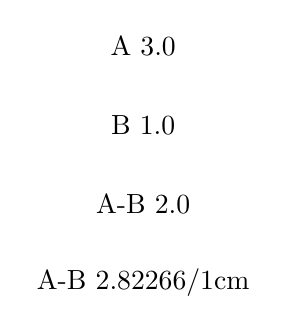
\begin{tikzpicture}
    % 定义两个坐标点
    \coordinate (A) at (3, 4);
    \coordinate (B) at (1, 2);

    % 获取 A 和 B 的 x 分量
    \newdimen\xA
    \newdimen\yA
    \newdimen\xB
    \newdimen\yB
    \pgfextractx{\xA}{\pgfpointanchor{A}{center}}
    \pgfextracty{\yA}{\pgfpointanchor{A}{center}}
    \pgfextractx{\xB}{\pgfpointanchor{B}{center}}
    \pgfextracty{\yB}{\pgfpointanchor{B}{center}}

     % 去掉单位
     \pgfmathparse{\xA / 1cm}
     \let\xAWithoutUnit\pgfmathresult
     \pgfmathparse{\xB / 1cm}
     \let\xBWithoutUnit\pgfmathresult

    % 计算 x 分量之差
    \pgfmathsetmacro{\xDiff}{\xAWithoutUnit - \xBWithoutUnit}

    \pgfmathsetmacro{\len}{veclen(\xA-\xB,\yA-\yB)/1cm}

    % 在图中显示结果
    \node at (0, -2) {A  \xAWithoutUnit};
    \node at (0, -3) {B  \xBWithoutUnit};
    \node at (0, -4) {A-B  \xDiff};
    \node at (0, -5) {A-B  \len/1cm};


\end{tikzpicture}

\end{document}